\documentclass[a4paper, 12pt]{article}

%% Language and font encodings
\usepackage[T1]{fontenc}
\usepackage[utf8x]{inputenc}
\usepackage{natbib}
\usepackage[french]{babel}

%Demande de l'INSPE de pas d'hyphénation mais rend le texte non justifié...
%\usepackage[none]{hyphenat}

% À decommenter si obligatoire. À vérifier aurpès de Maria...
%\usepackage{helvet}
%\renewcommand{\familydefault}{\sfdefault}
%\usepackage{setspace}
%\onehalfspacing


%\usepackage{multirow}
%\usepackage{wrapfig} 
%\usepackage{subfig}
%\usepackage{picins}

% Defining colors
\usepackage{xcolor, colortbl}
% \usepackage{colortbl} % colorier des tableaux
\definecolor{deepblue}{rgb}{0.3,0.3,0.8}
\definecolor{darkblue}{rgb}{0,0,0.3}
\definecolor{deepred}{rgb}{0.6,0,0}
%\definecolor{iremred}{RGB}{204,35,50}% ROUGE IREM
%\definecolor{deepgreen}{rgb}{0,0.6,0}
%\definecolor{backcolor}{rgb}{0.98,0.95,0.95}


\usepackage{tabularx}
\newcolumntype{Y}{>{\centering\arraybackslash}X} % centrer des colonne de type X
\usepackage{arydshln} % lignes en pointillées


%
\usepackage{hyperref}
%
%\usepackage{tocloft}
%\usepackage{xparse}
%\usepackage{etoolbox}
%\urlstyle{tt}
\newcommand{\email}[1]{\href{mailto:#1}{\tt{\nolinkurl{#1}}}}

\usepackage[parfill]{parskip}
\usepackage{fancyhdr}
\usepackage{authblk}
\renewcommand\Authand{ et }			%franciser
\renewcommand\Authands{, et }		%franciser
%\usepackage{calc}
%\usepackage{inconsolata}
%\setlength{\headheight}{40pt}


%% Sets page size and margins
%\usepackage[a5paper,top=3cm,bottom=2cm,left=2cm,right=2cm,marginparwidth=1.75cm]{geometry}
%%%%%%écrire dans la marge
\usepackage[fulladjust]{marginnote}
\usepackage[a4paper,margin=2cm]{geometry}% À changer en 2.5 selon les demandes de Maria : obligatoire ?
\reversemarginpar
\newcommand{\idee}[1]{%
\reversemarginpar
\hspace{-0.4em}\marginnote{\footnotesize #1}%
}
\newcommand{\info}[1]{\normalmarginpar\marginpar{
  \textcolor{deepred}{\texttt{
  \begin{minipage}[t]{1.5cm}
    \begin{flushleft}
      \tiny #1
    \end{flushleft}
  \end{minipage}
  }}}}
  

%% Useful packages
%\usepackage{amsmath}

\usepackage{graphicx}
%\usepackage{subfig} 

% renommer les figures
%\addto\captionsfrench{%
%  \renewcommand{\listfigurename}{Liste des captures}%
%  \renewcommand{\figurename}{\textsc{Capture}}%
  %\renewcommand{\listtablename}{Nouveau nom}%
%}

%\usepackage{booktabs}
%\usepackage[colorinlistoftodos]{todonotes}
%---
%\usepackage[most,listings,breakable,theorems]{tcolorbox}  
%%%%%%%%%%%%%%%%%%%%%%%%%%%%%%%%%
% nomenclature
\usepackage[acronym,toc]{glossaries}
\loadglsentries[\acronymtype]{main-acro} % chargement du fichier caffa-acro.tex
\renewcommand*{\glstextformat}[1]{\textcolor{darkblue}{#1}}
\makeglossaries


%Mettre dans crochets: "number within=section," <- pour numérotation sous la forme section/soussection du code
% cf doc de tcolorbox ici (469p!) :
%http://texdoc.net/texmf-dist/doc/latex/tcolorbox/tcolorbox.pdf
%\newtcbtheorem[auto counter,list inside=cmb]{CMB}{Code \no}
%{top=-1.5mm,bottom=-2mm,fonttitle=\sffamily\bfseries,arc=0mm, colback=backcolor,colframe=iremred}%
%{code}%<-pour ref{code:...}
%%%
%%%%-----


%\newcommand{\ciitice}{\gls{cii} \gls{tice}}

%%%%-----------------------------
%           TITRE et h/b de page
%%%%-----------------------------
%\renewcommand{\headrulewidth}{0pt}

\title{{
\includegraphics[width=\linewidth]{res/inspe}}\\[2cm]
Écrit réflexif\\professeur stagiaire\\2021-2022 \\[4cm]
\textbf{Découverte d'une méthode de pédagogie tutorée}\\[2cm]
}
\vspace{2cm}

\author{Pascal Padilla -- Lyc\'ee Simone Veil, Marseille; \email{pascal.padilla@ax-aix-marseille.fr}}
%\affil[1]{}%
%\affil[2]{}%

\date{}


%%
%\fancyhead[C]{
\includegraphics[width=0.5 \linewidth]{espe}}
%\fancyhead[R]{\includegraphics[width=2.5cm]{LogoC2it_800.png}}
%\fancyhead[R]{}
\fancyhead[L]{}

\fancyfoot[L]{Pascal Padilla}
\fancyfoot[R]{Écrit réflexif 2021-22}
\renewcommand{\footrulewidth}{1pt}

\pagestyle{fancy}


\usepackage{lipsum}
\newcommand{\remplissage}{
  {\color{deepblue}\lipsum[1][1-10]}}


% Citations perso
\newcommand{\textcite}[1]{\og \textit{#1} \fg{}}


%%--##################################################
\begin{document}

\pagenumbering{roman}



\renewcommand{\labelitemi}{\textbullet}

%%--##################################################
\maketitle

\thispagestyle{empty}
%Page de titre

\newpage
%%--##################################################
\begin{abstract}

Merci à Nicole Mencacci pour son accompagnement.

\end{abstract}

\thispagestyle{empty}

%%--##################################################
\newpage
%sommaire
\tableofcontents

\thispagestyle{empty}

%%--##################################################
\newpage
%%--##################################################
%
%  				DEBUT du texte principal
%
%--##################################################

\clearpage
\pagenumbering{arabic}


\section{Présentation}



\subsection{Contexte d'enseignement}



Lauréat du concours du CAPES de Numérique et Sciences Informatique (NSI), je suis  cette année professeur stagiaire. Préalablement fonctionnaire de l'éducation nationale en tant que professeur en lycée professionnel (PLP) de mathématiques, sciences-physiques et chimiques, je bénéficie du statut de professeur stagiaires à \emph{temps complet}. C'est l'occasion pour moi de produire cet écrit réflexif qui se propose de décrire un dispositif pensé et mis en œuvre durant cette année dans la cadre du master 2 Métiers de l'Enseignent, de l'Éducation et de la Formation (MEEF).

En effet, cette année est pour moi très particulière puisque, outre la découverte d'une discipline nouvelle à enseigner, j'assiste en parallèle à certains cours du M2 MEEF avec des professeurs stagiaires à \emph{temps partiel} de NSI et sciences de l'ingénieur (SI). Bénéficiant d'une validation des acquis pour certaines unités d'enseignement (UE) ainsi que d'une dispense de cours, je travaille néanmoins sur la validation de l'UE 2, accompagné pour cela par Jean-François Herold.

J'enseigne à 18 heures dans le lycée Simone Veil de Marseille (13~013). Cet établissement de 850 élèves accueille les élèves de la seconde au BTS et admet une section professionnel.

Mon service est partagé entre :

\begin{description}
    \item[8 heures] d'enseignement de sciences numériques et technologie (SNT) auprès de quatre classes de seconde et
    \item[10 heures] d'enseignement de NSI auprès d'élèves de première et de terminale.
\end{description}

L'enseignement de NSI est un \emph{enseignement de spécialité} qui a vu le jour avec la \emph{réforme du baccalauréat général et technologique et du lycée} de 2018. Cette réforme, après une succession d'évolutions, de modification et d'ajustements, propose actuellement et jusqu'à nouvel ordre aux élèves de fin de seconde de choisir trois enseignements de spécialités parmi l'ensemble des enseignements disponibles sur leur secteur d'affectation. En fin de première, ces derniers conservent deux enseignements, qui seront évalués au baccalauréat par des épreuves ponctuelles, et arrêtent leur troisième spécialité qui sera évaluée au baccalauréat par le contrôle continu.
\\
En fin de seconde, lors du choix des spécialités libre a lui (et à sa famille) de reproduire les menus traditionnels tels que :

\begin{itemize}
    \item pôle scientifique type S avec les spécialités mathématiques, physiques et sciences et vie de la terre (SVT)
    \item pôle littéraire type L avec humanité, littérature et philosophie (HLP), langue, littératures et cultures étrangères (LLCE)
    \item pole économique et social type ES avec histoire géographie, géopolitique et sciences politiques (HGGSP), sciences économiques et sociales (SES).
\end{itemize}

Néanmoins d'autres voies sont possibles et désormais l'éducation physique et sportive (EPS), les sciences de l'ingénieur (SI), la musique, l'audiovisuel ou les sciences informatiques font leur apparition auprès des spécialités typées plus traditionnelles.



\subsection{Trois constats}



\paragraph{Des élèves qui ne se connaissent pas}
%
En tant qu'enseignants de spécialité, je constate que je me retrouve face à un groupe d'élèves dont les seuls moments partagés se font dans notre cours. 
\\
En effet, cette individualisation du choix couplée à la richesse de l'offre engendre une très grande variété de couplages sur les cohortes d'élèves de première et de terminale. Par exemple sur mon établissement qui propose 9 enseignements de spécialités, pas moins de 84 combinaisons différentes sont possibles. Sur ces deux niveaux, il n'existe donc plus de classe aux spécialités homogènes. C'est-à-dire qu'il n'existe plus de classes dont tous les élèves suivent les mêmes enseignements de spécialité. Les classes de spécialité sont donc devenues des \emph{groupes} de spécialités, et la très grande majorité de ces groupes sont constitués d'élèves provenant de classes différentes.
\\
Ce morcellement des classes implique que les élèves se retrouvant dans chaque groupe de spécialité se connaissent beaucoup moins. Ils ne se côtoient ensemble que pendant les heures consacrées à chaque enseignement de spécialité. Le parcours de chaque élève est donc fortement individualisé et les groupes de spécialité sont structurellement d'une constitution autre que celle de la classe entière ou de ses demi-groupes. Il me semble que le fonctionnement structurel induit par la \emph{réforme du baccalauréat général et technologique et du lycée} engendre une école cloisonnant l'individu plutôt qu'une école comme levier de promotion du collectif. 


\paragraph{Nécessité d'une pédagogie différenciée}
%
En tant qu'enseignant, nous sommes face au constat que notre enseignement doit être différencié. Certes, c'est un lieu commun pour les institutions et le monde de la recherche, mais concrètement, face aux élèves, la réalité est implacable : les élèves sont tous différents. Par leurs expériences vécues, leurs façons de vivre la classe, leurs intégrations dans le groupe ou encore leurs sensibilités. Il ne peux donc pas en être autrement sur leurs besoins ou leurs façons d'apprendre.
\\
Cette différenciation est relativement aisée à penser en enseignement d'informatiques. Les environnements de travail, qu'ils soient matériels ou numériques, aident à la rendre opérationnelle. Muni d'un ordinateur et d'un espace de travail, il est facile de proposer des activités adaptées aux besoins de chacun. C'est un gros travail de logistique et de création, mais ça ne pose pas de grosses difficultés conceptuelles.


\paragraph{Importance du socio-constructivisme}
%
Enfin, je suis un enseignant convaincu de l'importance pour l'apprentissage de la dimension sociale.  Pour un enseignant, il est moins efficace de transmettre un savoir que de le faire se construire par l'apprenant. Cette dimension constructiviste peut prendre plusieurs formes comme une situation problème particulièrement bien sentie et adaptée à l'élève ou encore comme une verbalisation ou une reformulation dans un contexte proche.
\\
Je trouve l'approche par situations problèmes délicate à mettre en œuvre. Il faut une disponibilité de l'élèves au moment de la rencontre. Il est aussi nécessaire de prendre en compte la zone proximale de développement de l'élève pour rendre la tâche tout à la fois accessible mais pas trop. Cette symbiose entre l'apprenant, le savoir et la situation me paraît trop difficile à penser en amont. 
\\
En revanche, le constructivisme peut aussi trouver sa réalisation par l'approche sociale. Cet aspect met en avant les besoins fondamentaux humains que sont l'échange, le partage, l'empathie ou encore le vivre ensemble. Le socio-constructivisme défend qu'un savoir se construit d'autant mieux s'il émerge d'interactions sociales. Je trouve cette approche pertinente pour plusieurs raisons. D'une part, en étant bien menée, l'apprenant se sent mieux dans un groupe qui devient de plus en plus bienveillant. D'autres part, en trouvant des dispositifs adaptés ne prétendant pas tout anticiper, cette démarche, plus aisée à mettre en œuvre, s'appuie sur la diversité des élèves, de leurs échanges et de leurs interactions.


\paragraph{Face à la contradiction}
%
Avec ma nouvelle discipline à enseigner et dans ce contexte de groupe de spécialité, j'ai été troublé par le fait que les élèves ne se connaissent pas. Cette individualisation des parcours et ce cloisonnement m'apparaît clairement contradictoire avec le socio-constructivisme si important pour l'apprentissage. Si les interactions entres les élèves sont minimales, il y a alors absence d'intérêt, d'échange ou de partage entre eux.
%
C'est pourquoi pendant l'année il m'est apparu primordial de favoriser les interactions entre les élèves.Il m'était nécessaire de mettre en œuvre un dispositif de pédagogie différenciée qui puisse promouvoir le collectif.



\section{Méthode Jigsaw}

\subsection{Description de la méthode}


Parmi les différentes méthodologie proposée de pédagogie différenciée, je me suis tourné vers une pédagogie de \emph{tutorat bidirectionnel}. 
\\
L'idée de tutorat est de créer des groupes d'élèves intégrant deux rôles asymétriques : l'élève \emph{tuteur}, qui transmet un savoir, et l'élève \emph{apprenant}, qui découvre le savoir transmis par son camarade.
% 
Mais cette asymétrie possède le risque de la stigmatisation. Qu'il soit étiqueté par ses camarades \emph{bon} ou \emph{mauvais}, la classe ne doit pas être le lieu de ses tensions. C'est pourquoi le dispositif de tutorat doit pour moi permettre à tous les élèves de tenir chacun des deux rôles. C'est cet aspect là du tutorat que l'on qualifie de \emph{bidirectionnel}.
\\
J'ai donc imaginé un dispositif qui ressemble beaucoup à la méthode \emph{jigsaw} apparue aux États-Unis dans les années 1970 pour faire face à la déségrégation.

L'idée est de partitionner une notion globale à enseigner en savoirs distincts puis d'organiser la séance en deux moments aux objectifs différents :

\begin{description}
    \item[moment de l'appropriation] Dans un premier temps, des groupes d'élèves sont constitués et chaque groupe a pour objectif de s'approprier un savoir. Chaque groupe possède un savoir différent à étudier. Durant ce moment, tous les élèves prennent connaissance au sein de leur groupe d'expert d'un savoir dont ils seront les tuteurs.
    \item[moment de la transmission] Dans un deuxième temps, on répartit tous les élèves dans d'autres groupes de façon à séparer les tuteurs. Les nouveaux groupes créés doivent posséder au moins un tuteur de chacun des savoirs concerné. Durant ce moment, chaque élève doit s'approprier l'ensemble des savoirs ce qui oblige chaque tuteur à exposer, expliquer et faire comprendre le savoir dont il est le garant.
\end{description}



\subsection{Mise en place du dispositif}



Comme on peut le constater, chaque élèves est à la fois tuteur d'un savoir et apprenant de l'ensemble des autres savoirs.

Ce dispositif :

\begin{itemize}
    \item permet une absence totale de stigmatisation entres élèves et 
    \item favorise un échange très fort entres élèves centré sur le savoir.
\end{itemize}

Lors de la mise en œuvre d'un tel dispositif, puisque le moment d'appropriation nécessite une grande autonomie des élèves, il est indispensable de créer ces premiers groupes de façon différenciées. Il faut des groupes d'experts en phase avec le savoir à s'approprier, et pour cela il faut que les élèves d'un même groupe aient des zones proximales de développement (ZPD) proches et sécantes entres elles.
\\
Un avantage de cette différenciation en amont des élèves est de se faciliter la répartition des savoirs entres les groupes puisqu'on s'autorise à avoir des savoirs de niveaux et de difficultés différentes.

C'est pourquoi, une première étape d'évaluation des élèves est indispensable. Lors de ce moment de la différenciation, je me suis efforcé de créer des groupes de niveaux en lien avec les prérequis nécessaires lors des moments suivants.

La méthodologie réalisée a donc été organisée en trois étapes :

\begin{description}
    \item[étape (a)] moment de la différenciation pour créer des groupes de niveaux,
    \item[étape (b)] moment de l'appropriation pour former les futurs tuteurs, par groupe de niveau, sur les savoirs à transmettre,
    \item[étape (c)] moment de la transmission pour que chaque élève transmette au sein de son groupe son savoir.
\end{description}


\begin{center}
    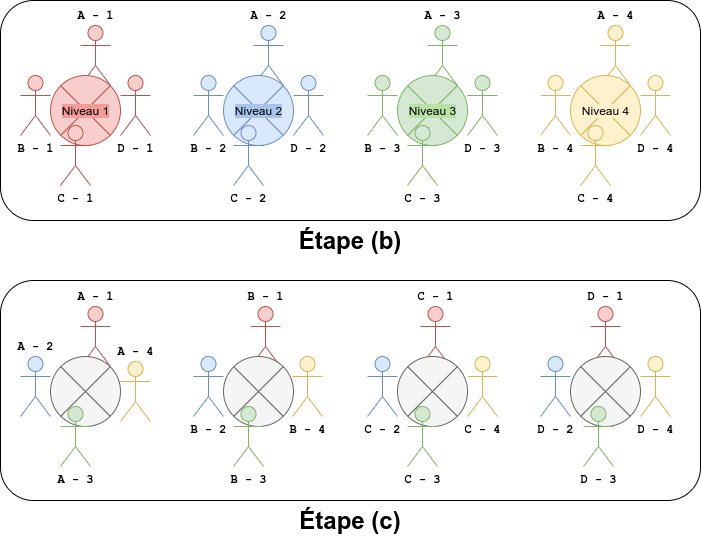
\includegraphics[width=0.75\linewidth]{res/diagramme.drawio.png}
\end{center}



\section{Première expérimentation}


J'ai procédé à ma première expérimentation au mois de mars. La notion globale travaillée concerne \emph{les types de base en informatique et la représentation des données en machine}.



\subsection{3 moments de la séances}



\paragraph{Moment de la différentiation}
%
J'ai listé les prérequis nécessaires au savoir global à enseigner lors de la séance tutorée. J'ai organisé ces prérequis en tâches puis j'ai organisé une première séance abordant chacune de ces tâches. À l'issue de cette séance, j'ai procédé à une évaluation des élèves pour créer des groupes de niveaux.
%
Pour faciliter la collecte des données et l'analyse à posteriori, j'ai décidé de travailler avec un outil dédié à l'enseignement en ligne : Moodle. J'ai proposé aux élèves une série de tests évaluant chacune des tâches identifiées.

Afin de ne pas pénaliser les élèves les plus lents et pour valoriser l'apprentissage des prérequis, j'ai autorisé pour chaque test un nombre illimité de tentatives. Mais afin de ne pas biaiser les résultats par des \emph{copier/coller}, j'ai mis en place des tests basés sur des valeurs aléatoires. C'est donc bien la méthode qui doit être correcte et non pas le résultat saisi ou coché.
%
Puisque le travail est en ligne, il a même été possible de demander aux élèves de finir le travail sur leurs temps personnels, en dehors de la classe. J'ai ainsi été conforté dans l'idée que les prérequis étaient assimilés.

À l'issue de cette séance, j'ai donc eu en ma possession une feuille de calcul indiquant pour chaque tâche, le niveau de réussite, le nombre de tentative et le temps passé par chaque élève.
%
Pour le moment de l'appropriation, j'ai besoin d'avoir des groupes homogènes. J'ai donc procédé à un classement des élèves par notes.
\\
Mais j'ai aussi voulu mettre en avant les élèves en fonction de leur degré d'autonomie. Pour cela, j'ai aussi pris en compte la durée totale nécessaire à l'achèvement d'une tâche donnée. Ainsi, mon classement final dépend de deux paramètres : le niveau de réussite et la vitesse de réalisation.

Pour chaque élèves, j'ai additionné pour chaque tâche son classement dans la classe et j'ai ainsi obtenu un score pour chaque élève. Plus ce score est petit, mieux l'élève a été classé en moyenne. Ce score m'a permis de créer trois groupes de niveaux nécessaire au moment de l'appropriation.


\paragraph{Moment de l'appropriation}
%
Quelques semaines plus tard, j'ai procédé au moment de l'appropriation. 

J'ai donc organisé les élèves par groupes, sans bien évidemment leur dire que c'était des groupes de niveaux. Chaque groupe a eu une feuille d'activité composée d'un savoir, de quelques exemples et d'une ou deux activités. Entres les groupes d'appropriation, les savoirs sont différents, mais chaque élève d'un même groupe travaille le même savoir.

L'objectif de chaque élève est de s'approprier le savoir, de comprendre les exemples et de savoir faire les activités. Pour cela, les échanges au sein du groupe d'experts sont encouragés ! Lors de la mise en activité, j'ai montré aux élèves la constitution des groupes de transmission à venir en leur indiquant l'objectif global de cette séquence de travail en groupe s'approprier un savoir pour le transmettre plus tard.

Dans les groupes, les élèves on naturellement commencé par lire leur document puis, après un moment de surprise et voyant que je n'intervenais pas, les échanges ont commencé dans les groupes.
\\
Ma posture a été d'intervenir le moins possible pour favoriser le partage et l'échange entre les élèves.


\paragraph{Moment de la transmission}
%
La séance suivante, j'ai mis en place les groupes de transmissions. Une même fiche d'activité est distribuée à chaque groupe. Cette fiche traite de la notion globale qui est constituée de l'ensemble des savoirs de chaque expert. L'objectif pour chaque élève a été clairement formalisé : expliquer aux élèves de son groupe sa notion experte. À la fin, chaque élève doit être capable de traiter seul la notion globale et la séance sera suivie d'un test de connaissance sur la notion globale.



\subsection{Observations et remarques}



\paragraph{Moment de le différentiation}
%
Ce moment a été le plus simple. Les élèves étant habitués à travailler sur Moodle, aucun n'a eu de difficulté pour se mettre au travail. L'activité étant réalisable un nombre illimité de fois, j'ai ajouté la note comme élément de motivation. J'ai indiqué aux élèves qu'il y aurait une note par tâche et que pour chacune d'entres elles, parmi toutes les tentatives réalisées, je garderai la note de celle la mieux réussie. Cet élément de note a été moteur pour inciter les élèves à mieux réussir et à recommencer si besoin leur travail. C'est aussi cet élément qui a fait que le travail a été fini à la maison par la plupart des élèves de la classe.
\\
L'analyse des résultats a été réalisée très simplement au tableur.


\paragraph{Moment de l'appropriation}
%
Pour des raisons externes, ce moment s'est déroulé longtemps après le moment précédent. Les prérequis travaillés préalablement étaient oubliés pour de nombreux élèves. Heureusement le travail en groupe a permis à certains d'expliquer à leurs camarades. Mais il y a eu des groupes qui avaient de gros manques.
\\
Certains élèves absents lors du moment de la différentiation ont été réparti dans les groupes les plus faibles car ils n'avaient pas travaillé les prérequis. Ce manque leur a été préjudiciable dans la phase d'appropriation car certains éléments leur échappaient complètement.
\\
L'absence d'autres élèves lors de ce moment m'a obligé à réorganiser les groupes en direct. À déplacer des élèves et à les changer de \emph{niveau}. Heureusement, et pour éviter la stigmatisation, j'avais préparé un tableau dynamique de groupe organisé en \emph{couleurs} et non en \emph{notes}.
\\
Je me suis rendu compte que j'ai mal évalué la durée de ce moment qui a pris beaucoup plus de temps que je ne le pensais. Je me suis adapté et n'ai pas interrompu le travail et les échanges entres les élèves. J'ai décidé sur le coup de reporter le moment de la transmission à la séance suivante. Ce choix était nécessaire mais a engendré certaines difficultés.
\\
Enfin, le plus gros problème rencontré est lié à mon attitude et à mon rôle durant ce moment : ma posture est à revoir. J'ai en effet décidé d'intervenir le moins possible, mais je me suis rendu compte lors de l'analyse des résultats que certains savoirs n'avaient pas été bien compris. Le problème est que si le savoir est mal interprété par les \emph{experts}, la transmission à venir est de piètre qualité, incomplète, voire erronée. Lors de mes prochaines séances, je pense faire le tour de tous les groupes et ajuster l'appropriation des savoirs.


\paragraph{Moment de la transmission}
%
Ce moment n'ayant pas eu lieu le même jour que le moment précédent, j'ai été confronté à l'absence d'un élève qui était présent précédemment. J'ai du modifier la constitution prévue des groupes. J'ai donc supprimé un groupe et ai réparti les élèves afin de d'avoir l'ensemble des savoirs pour chaque groupe. Cette adaptation a engendré des doublons d'experts.
\\
Par ailleurs, la séance a été interrompu au milieu par le départ de 25\% de mes élèves qui s'étaient inscrit à une présentation avec des intervenants extérieurs. Ce départ que je n'avais pas prévu m'a obligé à revoir la constitution des groupes. Il y a donc des experts qui ont dû expliquer plusieurs fois leurs notions. Il y a aussi des élèves qui, je m'en suis rendu compte après, n'ont pas eu d'explication sur un des savoirs.
\\
Par ailleurs, en voulant favoriser les échanges et en ne voulant pas supplanter le tuteur, je ne me suis rendu compte qu'à posteriori de l'incompréhension et de l'incapacité de certains tuteurs à transmettre une notion qui leur échappait complètement.



\section{Conclusion}



Après cette séquence, j'ai repris l'ensemble des savoirs en classe et les élèves ont retravaillé la notion globale. Ainsi, cette séquence n'est pas une fin en soi et on ne peut pas considérer la notion globale comme traitée suite à un tel dispositif.

Je n'ai pas encore évalué l'efficacité du dispositif au niveau des apprentissages. Néanmoins, je peux déjà apporter une première conclusion. Je trouve que cette expérience partagée par les élèves très enrichissantes pour eux. J'ai vu des élèves se parler et échanger pour la première fois. J'ai apprécier de voir que le savoir était au centre de leur préoccupation à ce moment là et c'était pour moi une expérience très agréable.

La création des fiches en amont a présenté un gros investissement et c'est le principal frein à ce genre de dispositif. En effet, pour chaque savoir il faut créer du contenu de cours, des exemples et des activités. Puis pour la notion globale, il faut créer deux fiches d'activités semblables mais différentes : l'une pour le moment de la transmission, une pour l'évaluation de la notion globale.
\\
Il y a donc beaucoup pour rendre de telles séquence opérationnelle. 

Néanmoins, sous réserve que les apprentissages ne soient pas (trop) dégradés, l'investissement me semble valorisant pour tous. Pour l'enseignant qui découvre une classe autonome et mobilisée et qui offre une expérience du vivre ensemble valorisante. Pour les élèves qui sont amenés à vivre un moment agréable de partage et d'échange centré sur le savoir.

% \thispagestyle{empty}\newpage

% \section{Constats et questionnements}

% Ordonnancement des idées :
\begin{enumerate}
	\item Groupes de spécialité et NSI
	\item Premier questionnement
	\item Groupe classe mal défini
	\item Pourtant socio-constructivisme
	\item Pédagogie différenciée
	\item Catégorisation de la pédagogie différenciée
	\item Notre dispositif
\end{enumerate}



La formulation explicite de notre question de recherche est le fruit d'une maturation lente. Dans cette partie, nous détaillons le cheminement de notre réflexion.


\subsection{Cadre socio-constructiviste}


%\idee{L'enseignement contemporain se fait dans un cadre constructiviste.}
\paragraph{Constructivisme}
Tout d'abord, notre mémoire se place dans le cadre du \emph{constructivisme}.
%
% \info{reformulation : ok}
%
Développée dès les années 1920 par Jean Piaget, qui la synthétise dans un de ses derniers ouvrages \citep{piaget_prise_1974}, cette théorie de l'apprentissage part du principe qu'un savoir ne se transmet pas ipso facto par l'enseignant, mais qu'il se construit par l'apprenant. Là où des théories comme le béhaviorisme prônaient l'inné face à l'acquis et l'apprentissage comme un réflexe face à un stimuli, le constructivisme propose quant à lui d'étudier l'activité du sujet en train de construire sa représentation mentale de la réalité. 
\\
Pour nous, cela se traduit par l'évidence qu'un cours n'est rien s'il ne permet pas une mise en activité de l'élève. Expérimenter, chercher, questionner, formuler, comprendre plutôt qu'apprendre, écouter ou noter.
%
D'ailleurs nos référentiels n'expriment pas autre chose et dire de l'élève qu'il est un acteur actif au centre de son apprentissage est désormais un point de vue que nous imaginons bien ancré et assimilé par le corps enseignant.



%\idee{Notre pratique quotidienne est ancrée dans un cadre socio-constructiviste.}
\paragraph{Socio-constructivisme}
Pour être plus précis, notre mémoire se place dans un cadre \emph{socio-constructiviste}.
%
\info{reformulation : OK\\Ajouter Vygotsky ! $\rightarrow$  Garnier, C., Bednarz, N. \& Ulanovskaya, I. (2009). Après Vygotski et Piaget: Perspectives sociale et constructiviste. Louvain-la-Neuve: De Boeck Supérieur.}
%
% Confronter les points de vue pour améliorer le sien et améliorer ses connaissances.
% Un tiers en réussite, un tiers moyen, un tiers en difficulté -> hétérogénéité "parfaite"
% Classes de niveau -> échec
% Vygotsky ? -> ZPD
% Roux, 1999
% Piaget : "Réussir et comprendre, c'est 2 choses différentes"
Découlant des travaux de Piaget, ce cadre a été développé par Willem Doise et Gabriel Mugny en \citeyear{doise_developpement_1981} et  \citeyear{doise_psychologie_1997}. Cette théorie se propose d'élargir l'environnement de l'apprenant en y intégrant la dimension sociale. Les interactions entre élèves y sont vues comme un instrument pour l'enseignant qu'il peut mettre à profit pour une mise en action favorisant l'apprentissage, car confronter les points de vue permettrait d'améliorer le sien et donc d'améliorer ses connaissances.
\\
Malgré tout notre professionnalisme et notre enthousiasme, il faut bien reconnaître que si un élève contemporain tolère l'obligation d'aller à l'école, c'est d'abord et surtout pour y retrouver des camarades, échanger et partager plutôt que pour y apprendre, travailler et progresser\footnote{Affirmation issue de notre expérience personnelle d'enseignant \textbf{et} d'élève.}.
%
Notre enseignement ne peut négliger ce besoin naturel de sociabilisation et notre travail de recherche s'articule donc tout naturellement autour de pratiques qui mettent en avant et valorisent les interactions entre élèves.
\\
Le socio-constructivisme se base également sur les travaux de Lev Vygotski, pédagogue russe du début du XX\up{ème} siècle ayant théorisé le concept de \textit{Zone Proximale de Développement (ZPD)}, qui définit l'espace entre lequel un enfant sait résoudre une tâche tout seul (en autonomie) et sait la résoudre avec une aide. La principale difficulté soulevée par cette \textit{ZPD} réside dans le fait qu'une personne avancée dans un domaine doit savoir entrer dans la \textit{ZPD} de l'apprenant pour que ce dernier puisse apprendre. Ce n'est qu'en recouvrant les \textit{ZPD} de l'apprenant et de l'enseignant que l'apprenant peut apprendre.




\subsection{Cadre de la différenciation}

En plus du socio-constructivisme, notre mémoire se place dans le cadre des pédagogies différenciées.

\subsubsection{Nécessité d'une pédagogie différenciée}\label{Pédagogie différenciée}

%\idee{Un constat : pour l'institution, la pratique d'une pédagogie différenciée est nécessaire.}
\paragraph{Nécessité issue du monde institutionnel}
%
% \info{reformulation : ok}
%
En premier lieu, les références institutionnelles sur lesquels nous devons nous appuyer en tant enseignants en France pour construire nos enseignements demandent explicitement de différencier. Ces textes imposent aux enseignants des valeurs communes, comme par exemple la laïcité, et des pratiques communes comme la mise en place pour les élèves d'\textcite{un accompagnement pédagogique adapté aux besoins de chacun afin de favoriser la réussite de leur scolarité [\ldots] Des propositions de différenciations doivent permettre à chaque élève de maîtriser les compétences attendues} \citep{eduscol_accompagnement_2020}.
\\
Cette demande explicite de différenciation dans notre pédagogie concerne aussi bien le champ du handicap que celui de la psychologie ou encore du social et s'appuie sur un socle théorique fort.



%\idee{Observant des différences de rythmes entre enfants, certains pédagogues proposent de privilégier l'accompagnement individuel.}
\paragraph{Nécessité issue du monde de la recherche}
%
% \info{reformulation : ok}
%
Évoquons maintenant le monde de la recherche. Dès lors qu'ils se sont intéressés à l'apprenant, les chercheurs en pédagogie n'ont pu que constater les différences entres individus.
Ainsi dans la première moitié du XX\up{ème} siècle, Piaget parvient à définir quatre stades de développement de l'enfant. Il observe que ces stades dépendent de tranches d'âge mais n'interviennent pas à la même période pour chaque enfant. 
Déjà la question des différences de rythmes de développement et de compréhensions entre élèves est posée.
%
De son côté, Celestin Freinet prône des pédagogies centrées sur l'enfant plutôt que sur l'enseignant ce qui amène ses contemporains à comprendre qu'\textcite{il n'est pas possible de proposer des apprentissages uniformes pour tous les élèves d'une même classe}, et qu'\textcite{il faut plutôt se diriger vers des apprentissages semblables.} \citep{lautru_pedagogie_2019}



%\idee{La formalisation du concept de pédagogie différenciée comme un effort pour répondre à la diversité des élèves.}
\paragraph{Formalisation du concept}
%
% \info{reformulation : ok}
%
La formalisation du concept de pédagogie différencié n'est cependant apparue que dans les années 1970. Dans ses travaux, Louis Legrand la définit comme \textcite{un effort de diversification méthodologique susceptible de répondre à la diversité des élèves} \citep{legrand_differenciation_1986}.
\\
En pratique, la pédagogie différenciée consisterait selon lui à \textcite{utiliser toutes les ressources possibles pour permettre aux élèves de développer leurs connaissances, ce qui suppose la diversité des démarches mais aussi des outils} \citep{battut_comment_2009}.
%
Ainsi, l'enseignant doit pouvoir proposer à chaque élève des tâches différentes afin que chacun puisse acquérir les notions issues des programmes officiels. 



% \idee{Le concept de pédagogie différenciée concerne aussi les diversités entre collectifs comme les classes.}
% Pointer le fait qu'il y a la théorie et la pratique, que tout ça est difficile à mettre en œuvre au quotidien car les différences existent tout le temps et pour tout le monde, que ce soit au niveau individuel (différences de niveau, de compréhension) comme au niveau collectif (les classes sont toutes différentes entre elles) 



%\idee{La pédagogie différenciée est naturellement présente dans toute situation d'enseignement.}
\paragraph{Situation actuelle}
%
% \info{reformulation : ok}
%
De nos jours, la \textcite{pédagogie différenciée} apparaît comme évidente et il nous semble naturel de la voir présente dans toute situation d'enseignement. \textcite{[Elle] est une réalité quotidienne incontestable} \citep{perrenoud_pedagogie_1995} et \textcite{est toujours là d'abord, avant tout effort pédagogique particulier, comme une réalité sociologique observable} \citep{meirieu_pedagogie_1996}.



\subsubsection{Mise en action de la pédagogie différenciée}



%\idee{Parce qu'elle est par essence centrée sur la différence entre individus, la méthode unique et universellement efficace de pédagogie différenciée n'existe pas.}
\paragraph{Pas de méthode universelle}
%
% \info{reformulation : ok}
%
Dans ses travaux sur la pédagogie différenciée, \cite{perrenoud_pedagogie_1997} affirme que \textcite{le cercle de ceux qui y réfléchissent et tentent quelque chose s'élargit}. On ne peut que constater qu'\textcite{une large palette de démarches et de procédés [\ldots] pour que les élèves apprennent un ensemble de savoirs et de savoir-faire commun à tous} \citep{battut_comment_2009} est proposée.
\\
Malgré ce foisonnement, Philippe \cite{meirieu_pedagogie_1996} se demande \textcite{pourquoi [il est] si difficile de mettre en pratique ses convictions pédagogiques}. Il identifie et oppose alors \textcite{deux grands courants théoriques de la différenciation} :
%
\begin{itemize}
	\item le \textcite{diagnostic a priori} : courant dans lequel \textcite{l'éducateur cherche à atteindre une sorte de \emph{nature profonde} du sujet qui lui permet de le classer dans une catégorie pour laquelle il dispose d'un ensemble de solutions} et 
	\item l'\textcite{inventivité régulée} : courant dans lequel l'\textcite{[éducateur] prend des indices qui lui permettent seulement de statuer sur les besoins du moment et d'avancer une proposition particulière dont on ne sait jamais d'avance comment elle sera accueillie et quels effets elle produira}.
\end{itemize}
%
Dans cette catégorisation, nous retrouvons encore la distinction entre le béhaviorisme et le constructivisme initiée par Piaget. Tout comme son prédécesseur, Meirieu conclut que pour lui l'\textcite{inventivité régulée} est la méthode à suivre car plus \textcite{ouverte}.
%
Malgré cette indication, il ne pousse pas plus vers l'opérationnalisation de la pédagogie différenciée et ne propose aucune méthode permettant sa mise en pratique. Il analyse cependant que \textcite{le pédagogue \emph{[est]} enrichi ou meurtri de ses expériences passées}, et que c'est donc par l'expérience pratique et théorique que l'enseignant pourra trouver la solution au problème pédagogique de chaque moment.



%\idee{L'enseignant doit utiliser en classes des dispositifs diversifiés favorisant les interactions entres les élèves.}
\paragraph{Concrétisation et limites}
%
% \info{reformulation : ok}
%
\cite{perrenoud_pedagogie_1997} fait partie des chercheurs contemporains qui s'intéressent à la mise en œuvre concrète d'une pédagogie différenciée dans les salles de classe. Ses publications portent donc sur la façon d'outiller l'enseignant afin de lui permettre d'acquérir une expérience pratique étayée par des apports théoriques. Selon lui, \textcite{le vrai défi est d'imaginer les dispositifs favorisant des interactions entre élèves, dans le cadre de divers groupes de travail, sans empêcher une individualisation du parcours de chacun}.\info{battut ; perrenoud}

%
%\idee{Pratiquer la pédagogie différenciée sans hésiter à  abandonner ses objectifs les plus ambitieux.}
%
De nombreux freins existent quant à la pratique en classe de la différenciation pédagogique. Par exemple en privilégiant l'accompagnement individuel,  le risque existe pour l'enseignant de baisser ses exigences collectives afin de permettre au plus grand nombre d'avancer dans l'apprentissage. Mais avec sa volonté forte de rendre opérationnelle la pédagogie différenciée, Philippe Perrenoud propose de se déculpabiliser. Son conseil est ainsi de \textcite{tourner le dos aux objectifs les plus ambitieux, pour assurer au moins l'égalité des acquis minimaux}.




%\idee{L'individualisation peut avoir des effets pervers.}
%
% \info{reformulation : ok}
%
La mise en pratique de la pédagogie différenciée doit aussi s'accompagner de précautions. Dans ses écrits, \cite{feyfant_individualisation_2008} promeut une pédagogie différenciée qualifiée d'\emph{individualisée} tout en mettant en garde les enseignants sur \textcite{l'individualisation [qui] peut prendre de multiples formes et avoir des effets bénéfiques ou à l'inverse stigmatiser et creuser les différences et les inégalités}. Dans un écrit plus récent, Annie Feyfant propose encore une autre précaution qui est de conduire une différenciation pour l'élève et non pour l'enseignant. Ainsi, l'\textcite{l'objectif n'est pas tant de différencier \emph{en soi} que la nécessité d'accompagner au mieux les élèves dans leurs apprentissages} \citep{feyfant_differenciation_2016}.




\subsection{Groupes de spécialité : individualisation et individualisme}


%\idee{Un constat : les groupes d'enseignement de spécialité sont constitués d'élèves provenant de classes différentes.}
\info{À revoir si on le déplace}Après avoir spécifié notre cadre d'étude, intéressons-nous maintenant à notre discipline : la \gls{nsi}.
\paragraph{Enseignement de spécialité et morcellement des classes}
%
% \info{reformulation : ok}
%
Depuis 2018 et la \emph{réforme du baccalauréat général et technologique et du lycée}, les enseignements de spécialités ont vu le jour, dont celui de \gls{nsi}. Pour son passage en classe de première, en dehors des disciplines du tronc commun, un élève de lycée général doit désormais choisir trois spécialités parmi l'ensemble des enseignements disponibles sur son secteur d'affectation. Cette individualisation du choix couplée à la richesse de l'offre engendre une très grande variété de couplages sur les cohortes d'élèves de première et de terminale\footnote{Par exemple avec 9 spécialités proposées sur un lycée, il y a théoriquement 84 combinaisons possibles de spécialité en première.}. Sur ces deux niveaux, hormis quelques exceptions et par volonté institutionnelle de ne pas recréer des classes de spécialité (quand bien même plusieurs élèves suivraient les mêmes spécialités), il n'existe donc plus de classe aux spécialités homogènes. C'est-à-dire qu'il n'existe plus de classes dont tous les élèves suivent les mêmes enseignements de spécialité. Les classes de spécialité sont donc devenues des \emph{groupes} de spécialités, et la très grande majorité de ces groupes sont constitués d'élèves provenant de classes différentes.



%\idee{L'individualisation induite par un groupe de spécialité constitué d'une somme d'individus qui ne partagent pas d'autres moments ensembles nous pose problème.}
\paragraph{Individualisation des parcours}
%
% \info{reformulation : ok}
%
Ce morcellement des classes implique que les élèves se retrouvant dans chaque groupe de spécialité se connaissent beaucoup moins. Ils ne se côtoient ensemble que pendant les heures consacrées à chaque enseignement de spécialité.  Le parcours de chaque élève est donc fortement individualisé et les groupes de spécialité sont structurellement d'une constitution autre que celle de la classe entière ou de ses demi-groupes.
\\
Cette individualisation des parcours et ce cloisonnement de l'élève nous interpellent fortement.
%
D'abord le travail extra-scolaire des élèves est fortement impacté. Prenons l'exemple de la réalisation d'un projet par des élèves. L'implication du groupe de projet en dehors des heures d'enseignement de spécialité est fortement entravée pour de simples raisons d'organisation, car les emplois du temps diffèrent et les créneaux libres ne se chevauchent plus.
%
Ensuite, cette diminution du temps personnel que nous venons d'évoquer a pour conséquence qu'un élève studieux aura moins de temps pour ce qui aurait été auparavant dévolu à des activités extra-scolaires lui permettant de se construire humainement et/ou de décompresser de la charge mentale du temps scolaire.
%
Enfin, dans notre société qui exacerbe l'individualisation, il nous semble essentiel de travailler sur la promotion du collectif. À ce titre, il nous apparaît que le fonctionnement structurel induit par la \emph{réforme du baccalauréat général et technologique et du lycée} engendre une école cloisonnant l'individu plutôt qu'une école comme levier de promotion du collectif. 

Comme le dit Gilles Monceau au sujet de la manière de voir les parcours scolaires et les apprentissages : \textit{aujourd'hui, c'est l'individualisation qui s'impose progressivement comme une nécessité et une évidence} \citep{monceau_groupe_2005}. Mais ce constat est extrêmement déstabilisant pour nous puisque les contenus des référentiels le contredisent et mettent en avant, par exemple, les compétences transversales de collaboration, de travail en équipes ou encore d'échanges !



%\idee{Notre intuition de professeur stagiaire est de vouloir recréer un vécu partagé entre les élèves, comme cela était le cas avant la création des enseignements de spécialité.}
\paragraph{Première intuition}
%
% \info{reformulation : ok}
%
En tant qu'enseignants de spécialité, nous nous retrouvons donc face à un groupe d'élèves dont les seuls moments partagés se font dans notre cours. 
%
Cet état des lieux nous interpelle car il apparaît en contradiction avec le cadre socio-constructiviste. Une première intuition a donc été de nous dire que cette méconnaissance des élèves les uns envers les autres n'est pas bénéfique pour leurs apprentissages. Si les interactions entre les élèves sont minimales, il n'y a alors ni échange, ni partage ou encore absence d'intérêt les uns pour les autres.
%
Au-delà de la mise en activité par le travail scolaire, il nous semble donc essentiel de favoriser aussi les interactions entre les élèves. En ce sens et puisque la notion de classe n'existe plus, notre idée a été de vouloir chercher les moyens de favoriser l'émergence d'un groupe, d'un collectif. Nous imaginons que l'expérience d'un vécu partagé et la connivence entre élèves seront quant à eux favorables aux apprentissages.



\subsection{Premier questionnement}


%Travailler dans un cadre différencié est aussi un thème fort des théories de l'enseignement. Comme nous venons de lele montre notre analyse dans la partie \ref{Pédagogie différenciée}, le monde de la recherche se penche sur cette question depuis près d'un siècle et une conclusion commune émerge qui tient sur l'évidence de construire des enseignements différenciés, quelle que soit la forme qu'ils prennent.




%\idee{Notre questionnement initial est donc de savoir comment concilier les deux constats précédents avec le socio-constructivisme.}
%Mais avant d'étudier plus attentivement cette nécessité d'une pédagogie différenciée, faisons le point sur l'état de notre réflexion initiale. 
%
% \info{reformulation : ok}
%
Après quelques semaines de travail, notre intuition de professeurs stagiaires nous est apparue antagoniste avec les deux constats précédents. C'est-à-dire que vouloir promouvoir le commun et le collectif pour un meilleur apprentissage nous a semblé contradictoire avec les évidences que (1) les groupes de spécialité sont formés d'élèves provenant de classes différentes et que (2) les institutions, tout comme la recherche, promeuvent la pédagogie différenciée.
%
C'est ainsi que notre questionnement s'est dans un premier temps formulé ainsi  : \emph{comment proposer une pédagogie différenciée à des élèves qui ne se connaissent pas, tout en partageant et échangeant collectivement ?}





\subsection{Le groupe classe, c'est quoi ?}
% Travail de groupe : Environnement socio-cognitif (cerveaux en interaction) susceptible de générer des progrès individuels.
%-> Effets positifs sur la dynamique de chaque individu
%-> Effets positifs sur la représentation de la tâche (on se perd moins).
%-> Déstabilise les procédures résolutoires individuelles (permet de ne pas s'enfermer dans sa procédure). Attention à ne pas trop guider pour permettre cette déstabilisation.
%-> Effets positifs sur le contrôle de l'activité.
%-> Confrontations efficaces
% Vygotsky
% Roux, 1999
% Baudrit, 2007

% Formes de travaux de groupe : collectif, collaboratif, coopératif, tutorat entre pair
% -> Attention à la constitution, au rôle et à la tâche du groupe.

% Constitution et rôle : interdépendance fonctionnelle (collaboration plutôt que coopération car besoin de mise en commun plutôt que somme d'individualité), hétérogénéité mesurée (des groupes de niveaux différents mais pas de trop gros écarts -> les zones proximales de développement doivent se superposer, cad qu'il faut que chacun puisse savoir se mettre au niveau de l'autre), égalité des statuts (un rôle pour chaque membre pour que chacun trouve sa place, sans "chef").
% Exemple de contrainte : que des classes différentes au sein du groupe.

% Temps consacré au travail de groupe ?
% Comment susciter la mise en commun ?

%\idee{La notion de groupe classe est mal définie par la recherche.}
\paragraph{Recherche d'une définition}
%
% \info{reformulation : ok}
Pour répondre à ce questionnement initial, et plus particulièrement pour formaliser le support de l'échange collectif entre élèves, nous avons mené nos premières recherches autour de la notion de \emph{groupe classe}. Contrairement à nos attentes, il se trouve que cette notion est assez mal définie et peu étudiée par le monde de la recherche. Malgré un usage très courant, nos recherches documentaires académiques et institutionnelles se sont vite montrées infructueuses.
\\
Lorsque \cite{peeters_contribution_2018} s'interroge sur la gestion des situations difficiles pour l'enseignant, il détaille les différents niveaux de fonctionnement d'un groupe ainsi que les moyens d'améliorer l'esprit de groupe. Mais il ne définit pas ce qu'est un groupe classe.
%
Même si les questionnements de \cite{monceau_groupe_2005} autour de la sociabilisation engendrée par des regroupements d'élèves en classes et ses réflexions politiques issues de ces questionnements nous ont semblé intéressants, il n'est pas question dans son article \emph{Groupe classe et groupes dans la classe} de définir formellement ce qu'est un groupe classe.
%
%: \textcite{L'hétérogénéité des classes [\ldots] assure de meilleures conditions de réussite pour les élèves les plus en difficulté scolaire [et pourtant] l'École a également produit, au fil de son histoire, des classes dites \emph{spéciales} qui reçoivent les élèves en difficulté dans les classes ordinaires. [\ldots] Bien des études ont montré que ces classes spéciales constituent des filières dont les élèves s'échappent rarement, bien que l'intégration soit souvent le mot d'ordre de ces dispositifs. Ce choix politique [est donc] de scolariser séparément certains élèves qui ne sont pas et ne seront plus jamais \emph{à l'heure\footnote{Par le terme \emph{à l'heure}, Monceau évoque la progression d'un élève par rapport aux attentes de l'institution en fin d'année de son niveau de classe.}}.} \citep{monceau_groupe_2005}
\\
%En dehors des réflexions de Monceau, nous n'avons pas trouvé d'autre contribution théorique à la définition de la notion de groupe classe.
Ainsi nous n'avons pas trouvé de contribution théorique définissant explicitement la notion de groupe classe.


%\idee{Nous postulons que l'expérimentation d'un vécu pédagogique partagé est bénéfique pour l'apprentissage des élèves.}
\paragraph{Un vécu partagé est bénéfique}
%
% \info{reformulation : ok}
%
Il n'a pas été possible pour nous d'analyser formellement les bienfaits apportés par un vécu partagé au sein du groupe classe. D'abord, comme nous venons de le voir, à cause du manque de précision de la notion de \emph{groupe classe}. Mais aussi face au manque de ressources traitant des bienfaits induits par l'expérience d'un \emph{vécu partagé}.
%
Même si, dans le but de faciliter la gestion de groupe, \cite{peeters_contribution_2018} donne des pistes pour améliorer \textit{le bon esprit ou [la] cohésion de groupe}, il n'analyse pas dans son article les bénéfices ou les bienfaits que l'enseignant peut en tirer pour l'apprentissage des élèves.
%
Toutefois, inspirés par les effets positifs du socio-constructivisme, nous sommes convaincus qu'il est bénéfique pour l'apprentissage des élèves de créer puis de leur proposer des situations permettant d'avoir en commun un vécu pédagogique partagé.



%\idee{Analyser quantitativement l'émergence d'un vécu partagé nous semble difficile puisque celle-ci apparaît dans tous les cas : qu'elle soit naturelle ou forcée par l'enseignant.}
\paragraph{Quantification du vécu partagé}
%
% \info{reformulation : ok}
%
Face à ce postulat, et malgré l'absence de preuve de son intérêt pour l'apprentissage, nous avons commencé à établir une mesure de la connaissance que les élèves ont de leurs camarades. Nous leurs avons proposé un premier questionnaire en début d'année. Notre objectif était de les interroger ainsi à intervalle régulier avec l'idée d'analyser l'évolutions des différents résultats en prenant pour variable le type d'activités proposées selon qu'il favorise ou non l'émergence d'un vécu partagé.
%
Mais nous nous sommes rendus compte que cette démarche ne peut pas prouver que notre dispositif conduit à l'émergence d'un vécu partagé. En effet, le type d'activité ne constitue pas à lui seul la seule variable permettant aux élèves de se connaître
et l'intensité de son influence reste bien minime face à tous les échanges ayant lieu en dehors de ce moment. Il est ainsi évident que la connaissance des élèves entre eux s'améliore nécessairement au cours de l'année et ce, que l'on intervienne ou non dans le processus de connaissance. Notre questionnaire n'aurait pas pu rendre compte de l'importance du type d'activités sur ce phénomène.









\subsection{Émergence de notre dispositif de pédagogie différenciée}

%\idee{Notre recherche s'oriente vers la mise en place d'un dispositif opérationnel concilliant toutes les réflexions précédentes.}
\paragraph{Synthèse des réflexions}
%
% \info{reformulation : ok}
%
L'ensemble de nos recherches et de nos réflexions nous mène à faire évoluer notre questionnement. Nous cherchons donc à mettre en œuvre un dispositif opérationnel de différenciation engendrant le moins possible d'effets pervers dus à la nécessaire individualisation, elle-même accentuée par le morcellement des classes en groupes de spécialité.



%\idee{Une partition des dispositifs différenciés en quatre catégories : le plan de travail, la table d'appui, les groupes de besoins et le tutorat entre élèves.}
\paragraph{Catégorisation des dispositifs de pédagogie différenciée}
%
% \info{reformulation : ok}
%
La recherche de notre dispositif différencié a été facilitée par l'organisation des nombreuses mises en œuvres possibles en quatre catégories. Face aux \textcite{réponses concrètes [qui] demeurent quant à elle plurielles}, \cite{forget_penser_2018} propose de classer les dispositifs de pédagogie différenciée en quatre catégories :
% Ces dernières peuvent être complémentaires et peuvent se concrétiser pendant les trois moments qui sont \textit{avant, pendant et après l'enseignement} :

\begin{description}
	\item [Le plan de travail] qui consiste à construire des progressions individuelles en laissant chaque élève accomplir les tâches d'enseignement à leurs rythmes. Cette catégorie promeut l'\textit{autogestion} de l'élève dans son apprentissage.
	\item [La table d'appui] qui est un lieu au sein de la classe où l'élève peut obtenir une aide à la réalisation de la tâche d'enseignement.
	\item [Les groupes de besoin] qui proposent à tous les élèves (et pas seulement à ceux qui sont le plus en difficulté), des tâches adaptées aux besoins du moment vis-à-vis de l'avancement de leur apprentissage.
	\item [Le tutorat entre élèves] qui propose aux meilleures élèves d'aider les élèves les plus en difficulté sous forme de tutorat en couple.
\end{description}



% La recherche de ce dispositif s'est concrétisée par la lecture d'ouvrages proposant différentes formes de mise en pratique de la pédagogie différenciée. Parmi celles-ci, la synthèse d'nous a paru la plus intéressante à creuser. Dans cet ouvrage, Forget, après avoir rappelé que \textit{les auteurs s'accordent sur les définitions générales de la différenciation pédagogique} mais que \citep[p.18]{forget_penser_2018}, propose de partitionner les dispositifs de pédagogie différenciée en quatre catégories, qui peuvent être complémentaires, à concrétiser pendant les trois temps de l'enseignement, à savoir \textit{avant, pendant et après l'enseignement} (Ibid, p.45) :
% \begin{itemize}
% 	\item Le plan de travail, qui consiste à construire des progressions individuelles en laissant chaque élève accomplir les tâches d'enseignement à leurs rythmes. Cette catégorie promeut l'\textit{autogestion} de l'élève dans son apprentissage.
% 	\item La table d'appui, qui consiste à proposer un lieu au sein de la classe où l'élève peut obtenir une aide à la réalisation de la tâche d'enseignement.
% 	\item Les groupes de besoin, proposant à tous les élèves (et pas seulement à ceux qui sont le plus en difficulté), des tâches adaptées aux besoins du moment vis-à-vis de l'avancement de leur apprentissage.
% 	\item Le tutorat entre élèves, proposant aux meilleures élèves d'aider les élèves les plus en difficulté sous forme de tutorat en couple.
% \end{itemize}






%\idee{Parmi ces catégories, nous choisissons de nous orienter vers le tutorat entre élèves}
\paragraph{Tutorat entre élèves}
%
% \info{reformulation : ok}
%
Après avoir analysé le partitionnement proposé par \cite{forget_penser_2018}, il nous est rapidement devenu évident que le dispositif différencié correspondant le mieux à nos besoins est celui du \emph{tutorat entre élèves}.
\\
Il permet de répondre au problème d'individualisation tout en proposant un cadre socio-constructiviste fort. Toutefois, sensibilisé par les méfaits de la stigmatisation, une mise en œuvre naïve qui définirait quelques élèves \emph{tuteurs} et les autres \emph{apprenants} nous semble contre productive. C'est pourquoi le point central de notre dispositif est de permettre à tous les élèves, y compris ceux le plus en difficulté, d'être tantôt l'apprenant et tantôt le tuteur source du savoir pour ses camarades. La transmission du savoir entres les élèves se faisant dans les deux sens, notre dispositif sera donc un tutorat \emph{bidirectionnel} entre élèves.

Il nous faut maintenant faire face à de nombreuses difficultés. Comment former des groupes d'élèves ayant des zones proximales de développement sécantes ? Est-il possible de rendre tous les élèves tuteurs ? 


% L'analyse de ces différentes catégories nous a amenés à nous questionner sur celle que nous allions privilégier. Le tutorat entre élèves est très vite apparu comme évident à nos yeux, car il permet de répondre au problème d'individualisation en forçant l'échange entre élèves, et surtout de mettre en pratique le socio-constructivisme de Vygotsky, la plus grosse difficulté étant de former des couples d'élèves ayant une \textit{zone proximale de développement} similaire. Ces quatre catégories comportaient toutes un gros risque de stigmatisation entre les \og bons \fg{} et les \og moins bons \fg{}. Il nous a semblé être plus facile de contourner ce problème grâce au tutorat entre élèves, car nous savions que nous pourrions trouver, même chez les élèves les plus en difficulté, un point sur lequel ils pourraient apporter aux élèves en ayant moins.

\vspace{1cm}

{\Huge FIN ?}

\subsection{Pédagogie de tutorat bidirectionnelle}
%\idee{Nous nous proposons donc d'utiliser la notion de pédagogie différenciée pour construire une pédagogie collaborative permettant à tous les élèves d'apporter chacun leurs compétences.}
\paragraph{Pédagogie différenciée collaborative}
Partant des constats et réflexions menés jusqu'à présent, nous avons réfléchi à une méthode de tutorat entre élèves qui serait collaborative, mais surtout qui inclurait tous les élèves quels que soient leurs niveaux. Nous voulions éviter de stigmatiser certains élèves en proposant un tutorat unidirectionnel où les \og meilleurs \fg{} aident les \og moins bons \fg{}. C'est en commençant à construire cette méthode que nous nous sommes aperçus qu'elle ressemblait grandement à la méthode Jigsaw.

%\idee{Jigsaw est apparu dans les années 1970 au USA, en pleine période de déségrégation raciale.}
\paragraph{Histoire de Jigsaw}
Cette technique d'enseignement a été créée dans les années 1970 par Elliot Aronson, actuellement Professeur à l'Université de Californie à Santa Cruz. À cette époque, la déségrégation venait de débuter dans les écoles américaines, et les jeunes américains issus des communautés blanches, noires et hispaniques se sont retrouvés pour la première fois ensemble en classe. Après quelques semaines, la peur et le manque de confiance entre les groupes d'élèves commençaient à créer des tensions. Il fallait donc trouver une solution pour faire en sorte que les groupes d'élèves s'entendent entre eux.


%\idee{Jigsaw est une technique d'enseignement coopérative qui promeut l'écoute, l'engagement, l'interaction et le partage.}
\paragraph{Présentation de la méthode Jigsaw}
Aronson a donc imaginé et mis en place la méthode Jigsaw : le but était que pour chaque notion du programme, celle-ci soit découpée en tâches essentielles à la compréhension de la notion, et que chaque tâche soit étudiée par un élève issu d'une communauté différente. Ainsi, chaque élève \og expert \fg{} de sa tâche est essentiel à la compréhension de la notion par tout le groupe. Cette technique a ensuite été généralisée pour ne plus seulement travailler la déségrégation, mais plus globalement pour permettre à chaque élève d'apporter quelque chose au groupe, pour ainsi se sentir moins seul et moins exclu. La mise en place d'une telle technique permet également aux élèves de développer des compétences humaines telles que l'écoute et le partage, car chaque élève doit apprendre et enseigner à l'autre pour acquérir la notion dans sa globalité.

Concrètement, Jigsaw se décompose en 10 étapes :
\begin{enumerate}
	\item Créer des groupes Jigsaw de 5-6 étudiants de niveaux, genres et origines hétérogènes.
	\item Nommer un leader pour chaque groupe, qui sera chargé de médiation au sein du groupe.
	\item Diviser la leçon du jour en autant de sous-leçons qu'il y a d'étudiants au sein de chaque groupe.
	\item Assigner une sous-leçon à chaque membre du groupe.
	\item Laisser à chaque étudiant le temps de se familiariser avec sa sous-leçon (au moins 2 lectures du thème).\label{Familiarisation}
	\item Former des \emph{groupes d'experts} en regroupant les étudiants ayant la même sous-leçon à étudier. Laisser à chaque groupe d'experts le temps d'échanger sur la sous-leçon afin de pouvoir tous présenter le même contenu aux groupes Jigsaw.
	\item Reformer les groupes Jigsaw.
	\item Demander à chaque étudiant de présenter la sous-leçon dont il est expert à son groupe.\label{PrésentationSousLecon}
	\item Naviguer entre les groupes pour observer et éventuellement intervenir en cas de problème.
	\item Évaluer les étudiants sur la leçon dans sa globalité.
\end{enumerate}

%\idee{Notre méthode de tutorat bidirectionnel est proche de celle de Jigsaw}
\paragraph{Notre Jigsaw}
Instinctivement, nous avions imaginé une méthode extrêmement proche de Jigsaw, et le fait que Jigsaw existe nous a conforté dans notre idée qu'elle pourrait permettre de répondre à nos attentes. Notre méthode, présentée sur la figure \ref{SchémaNotreJigsaw}, diffère de Jigsaw sur plusieurs points :
\begin{itemize}
	\item Pour des questions d'effectifs et de décomposition des leçons que nous avons choisies, nos groupes Jigsaw ne sont composés que de 3 à 5 élèves.
	\item L'hétérogénéité de nos groupes Jigsaw n'est basée que sur les niveaux des élèves, ayant très peu de filles et n'ayant pas suffisamment d'origines ethniques différentes.
	\item Nous ne nommons pas de leader dans les groupes Jigsaw, voulant appuyer le côté collaboratif et ne voulant pas valoriser certains élèves au détriment d'autres.
	\item Nous n'effectuons pas l'étape \ref{Familiarisation}, par manque de temps pour chaque séance et considérant que le côté familiarisation est effectué à l'étape suivante de manière collective.
	\item L'étape \ref{PrésentationSousLecon} consiste en la résolution par le groupe Jigsaw d'un exercice pour chaque notion issue de chaque sous-leçon.
\end{itemize}


\newpage

\newgeometry{margin=2cm,left=5cm,marginparwidth=4cm}
\fancyhfoffset[L]{3cm}



\subsection{Idées non classées pour le moment mais qui peuvent s'avérer intéressantes}


\idee{Dans la pédagogie de tutorat, l'échange de savoirs entre élèves peut être vu comme la genèse instrumentale du savoir.} 
Le cadre théorique dans lequel nous nous inscrivons est celui de \cite{rabardel_les_1995} lorsqu'il distingue artefact et instrument. L'artefact est l'objet, l'outil ou dans notre cas la ressource mise à disposition par l'enseignant auprès du groupe d'appropriation. L'instrument est une entité composée de l'artefact, ou d'une partie de celui-ci, et la mise en action de ce dernier par l'élève, l'adaptation qu'il en fait pour l'accommoder à ses besoins lorsqu'il doit le transmettre à ses camarades.


\idee{La pédagogie différenciée contemporaine}
De nos jours, de nombreux travaux s'appuient sur ceux de Piaget et Freinet, pour proposer des solutions pratiques à la pédagogie différenciée. Bien différentes les unes des autres, ces études nous montrent bien qu'il n'y a pas de méthode miracle, mais que le plus important pour un enseignant est de se questionner quotidiennement sur l'efficacité des méthodes qu'il emploie et de s'adapter aux différentes situations de classe.





\idee{Kahn expose 3 grandes questions sur la différenciation}
Cette difficulté de pratique de la différenciation se retrouve chez \cite{kahn_pedagogie_2010}, pour qui la définition même de la pédagogie différenciée peut prêter à discussions. Elle expose trois grandes questions sur les conceptions contemporaines de la différenciation : 
\begin{itemize}
	\item \textcite{La pédagogie différenciée [\ldots] touche à la notion de différences entre les individus. [\ldots] L'école est aux prises avec des injonctions divergentes qui vont de la sacralisation de la différence à l'effort vers la construction d'une universalité.}
	\item \textcite{\emph{Se préoccuper} des différences entre élèves peut s'entendre en deux sens opposés : on peut vouloir les sauvegarder ou on peut vouloir les réduire.}
	\item \textcite{L'idée de \emph{traiter} les différences entre élèves [\ldots] peut se faire au niveau de l'institution elle-même par la diversification du cursus en filières différentes, [\ldots] entre les classes d'une même filière à l'échelle d'un établissement, [\ldots] au niveau des élèves d'une même classe en prévoyant pour certains d'entre eux des dispositifs de remédiation, [mais] aussi au sein même de la classe au moyen d'activités différentes selon les élèves.}
\end{itemize}



\idee{Cheminement de notre réflexion}
Parler de notre réflexion initiale sur l'appartenance au groupe classe, et la difficulté de mise en œuvre d'une pédagogie différenciée dans une classe avec des élèves qui ne se connaissent pas. Et notre bifurcation vers la pédagogie collaborative, que l'on pense être une forme de pédagogie différenciée qui peut répondre au problème de non-connaissance des élèves entre eux.

\newgeometry{margin=2cm}
\fancyhfoffset[L]{0cm}\newpage

% \section{Questions de recherche}

% À partir des réflexions menées pour affiner les questions que nous nous posions, la question que nous avons retenue est la suivante :

\textbf{Une pédagogie différenciée de tutorat entre élèves bidirectionnel permet-elle d'améliorer l'apprentissage en enseignement de spécialité ?}

De cette question découlent 2 hypothèses :
\begin{itemize}
	\item Un élève qui transmet une notion à ses camarades améliore ses apprentissages sur cette notion.
	\item Un élève qui reçoit une notion transmise par un camarade voit son apprentissage de la notion amélioré.
\end{itemize}

Cette forme pédagogie différenciée est à différencier de la notion de tutorat, pour lequel la transmission est unidirectionnelle. Ici la transmission est bidirectionnelle (les \og bons \fg{} transmettent aux \og moins bons \fg{} mais les \og moins bons \fg{} transmettent aussi aux \og bons \fg{}).\newpage

% \section{Méthodologie de recherche}

% 
Notre étude porte sur trois groupes d'élèves de premières de lycée général suivant l'enseignement de spécialité NSI.
Deux groupes sont au lycée Monte-Cristo d'Allauch. Chaque groupe est composé de 18 élèves (dont 1 fille et un élève sourd pour l'un et 2 filles pour l'autre).
Le troisième groupe est au lycée Simone Veil de Marseille. Il est composé de 14 élèves (dont 2 filles).

La principale difficulté de notre étude porte sur le fait que nous ne pouvons pas anticiper les retards et/ou absences des élèves sur notre séance Jigsaw, car la constitution des groupes de niveaux est à faire en amont de la séance. Ainsi, nous nous devons de prévenir les élèves que nous allons effectuer une séance particulière, et ils se mettent donc peut-être une pression supplémentaire sur cette séance extraordinaire, ce qui peut biaiser notre étude.

Pour quantifier une pédagogie différenciée collaborative, nous proposons de travailler de la façon suivante :
\begin{enumerate}
	\item enseigner une même partie du programme de deux manières différentes en fonction des groupes :
	\begin{itemize}
		\item 1 ou 2 groupes témoins : méthode classique (cours magistral, TD, TP, évaluation).
		\item 1 ou 2 groupes tests : méthode Jigsaw.
	\end{itemize}
	\item évaluation sommative sur les notions abordées (recueil de performances académiques).
	\item évaluer un mois plus tard chacun des groupes avec un même support pour chaque groupe.
	\item reproduire ces premiers points sur une autre partie du programme en inversant les groupes test et témoin.
\end{enumerate}

Les variables de notre étude sont donc principalement quantitatives. En parallèle de celles-ci, nous avons décidé de filmer les séances afin d'obtenir des données plus qualitatives (à revoir $\rightarrow$ va-t-on analyser qualitativement ?)

Tableau qui guide la logique de la recherche, ne pas le recopier dans le mémoire.

\begin{center}
\begin{tabular}{|c|c|c|c|c|}
	\hline
	& \multicolumn{2}{|c|}{Variable 1 (Jigsaw)} & \multicolumn{2}{|c|}{Variable 2 (Pas Jigsaw)}\\
	\hline
	& Qualitative & Quantitative & Qualitative & Quantitative\\
	\hline
	Performance &  & x &  & x\\
	\hline
	Tutorat entre pairs & x &  & x & \\
	\hline
	Sollicitation enseignant & x &  & x & \\
	\hline
	Engagement activité & x &  & x & \\
	\hline
\end{tabular}
\end{center}

\begin{figure}[h!]
	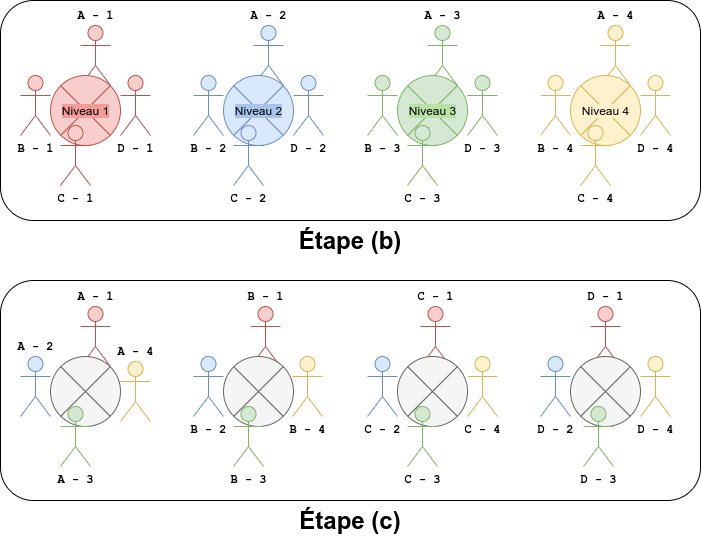
\includegraphics[width=\textwidth]{res/diagramme.drawio}
	\caption{Représentation de notre pédagogie collaborative}\label{SchémaNotreJigsaw}
\end{figure}

Nous avons choisi de travailler sur les deux notions suivantes provenant du programme officiel de première \gls{nsi} :
\begin{itemize}
	\item \emph{Représentation des données : types et valeurs de base} au sein de laquelle se trouvent les contenus suivants :
	\begin{description}
	    \item[Contenu 1] Écriture d'un entier positif dans une base $b=2$,
	    \item[Contenu 2] Écriture d'un entier positif dans une base $b>2$,
	    \item[Contenu 3] Représentation binaire d'un entier relatif,
	    \item[Contenu 4] Représentation approximative des nombres réels : notion de nombre flottant,
	    \item[Contenu 5] Valeurs booléennes, opérateurs booléens et expressions booléennes,
	    \item[Contenu 6] Représentation d'un texte en machine.
	\end{description}
	Nous avons choisi de retirer de notre étude les contenus 4 et 5 sur les notions booléennes, pour réduire le nombre de notions abordées lors de la séance Jigsaw et car nous avons considéré que ces notions peuvent être abordées dans une autre séquence.
	\item \emph{Constructions élémentaires des langages de programmation} au sein de laquelle se trouvent les contenus suivants :
	\begin{description}
	    \item[Contenu 1] Séquences d'instructions, variables et affectations,
	    \item[Contenu 2] Structures conditionnelles,
	    \item[Contenu 3] Structures itératives bornées,
	    \item[Contenu 4] Structures itératives non bornées,
	    \item[Contenu 5] Appels de fonction.
	\end{description}
	Nous avons choisi de retirer de notre étude le contenu 5 sur les appels de fonction, pour les mêmes raisons que précédemment.
\end{itemize}

\idee{Les contenus de programme étudiés lors des trois moments didactiques de notre méthodologie.}
Conformément à notre méthodologie, la séquence est partagée en trois moments didactiques distincts : le moment de la différenciation, le moment de l'appropriation et le moment de l'échange. 

Chacun de ces moments est l'occasion pour l'élève d'aborder les contenus de programme identifiés :

\begin{description}
    \item[Moment de la différenciation] qui permet à l'enseignant de créer trois groupes de niveau et à l'élève de (re)travailler les prérequis nécessaires lors des moments suivants :
    \begin{itemize}
        \item Contenu 1
    \end{itemize}
    \item[Moment de l'appropriation] qui permet à l'élève d'aborder un contenu adapté à son niveau parmi les trois possibles :
    \begin{itemize}
        \item Contenu 2 (pour un élève du groupe 1, niveau facile)
        \item Contenu 3 (pour un élève du groupe 2, niveau intermédiaire)
        \item Contenu 6 pour les types et valeurs de base, 4 pour les constructions élémentaires (pour un élève du groupe 3, niveau difficile)
    \end{itemize}
    \item[Moment de l'échange] qui permet à l'élève d'aborder les deux contenus du moment précédent qu'il n'a pas encore rencontré.
\end{description}

\idee{Des activités pour différencier les élèves.} 
L'objectif du moment de la différenciation est de créer des groupes de niveaux. L'intérêt de cette discrimination des élèves est de proposer lors du moment de l'appropriation un travail adapté au niveau de chacun.
\info{\#TODO ajouter une source théorique}
Ainsi à l'issue de notre séance chaque élève, quel que soit son niveau, aura été à fois récepteur mais aussi et surtout transmetteur de savoir-faire auprès de son groupe d'échange.

Pour différencier les élèves, nous utilisons des activités qui sont construites pour être réalisées par les élèves en autonomie. Ces activités nous permettent d'établir un diagnostic concernant l'aisance des élèves sur le contenu 1.

\idee{Décomposition des contenus du programme en tâches pour décrire le travail de l'élève}
Afin de mieux décrire le travail de l'élève à l'issue de ces activités, nous proposons une décomposition en tâches des contenus du programme abordées lors du moment de la différenciation. Cette décomposition en tâches permet donc de clarifier l'objectif de chacune des activités du moment de la différenciation.


% 
\subsection{L'appropriation \og classique \fg{} des notions : groupes témoins}

Tout d'abord, il convient de définir ce que nous concevons comme étant une appropriation \og classique \fg{} des notions. En effet, même s'il existe beaucoup de différences entre les pratiques pédagogiques, nous constatons qu'un courant pédagogique prédomine en France. Ce courant divise les séances de cours en quatre types : séance de cours, travaux dirigés (TD), travaux pratiques (TP) et évaluation. Bien entendu, au sein d'une même séance, plusieurs types peuvent être pratiqués. Chaque enseignant peut ainsi proposer à ses élèves différentes activités en fonction du type utilisé, mais cette grande catégorisation reste un commun dans l'enseignement français.

Nous nous proposons donc de définir comme groupes témoins les groupes pour lesquels les notions abordées l'ont été au travers de cette appropriation classique.


\subsubsection{Types et valeurs de base : groupes témoins}
Cette phase a été réalisée au sein de deux groupes témoins au lycée Monte-Cristo d'Allauch.

Il s'agissait de la première séquence de l'année, au cours de laquelle les élèves découvraient l'informatique en plus de leur enseignant et leurs camarades. La méthode \og classique \fg{} se retrouve dans la construction générale de la séquence, même si les parties cours et TD étaient quelque peu mélangées.

Cette séquence a duré un mois, période après laquelle la première évaluation sommative a été réalisée.

Il s'agissait tout d'abord de travailler au cours des premières séances sur le dénombrement, afin de pouvoir aborder l'écriture d'un entier en binaire. Le but était de faire prendre conscience aux élèves que le dénombrement décimal utilisé tous les jours n'est qu'une représentation comme une autre de nombres, qui peuvent ainsi être représentés différemment, comme en binaire ou en hexadécimal. C'est comme cela que ces représentations ont été introduites.

Par la suite, un document de cours contenant l'ensemble des notions de la séquence a été distribué, et chaque contenu a été abordé au cours de séances de TD pendant 4 à 6 heures chacun.

\subsubsection{Constructions élémentaires : groupe témoin}
Cette phase a été réalisée au sein d'un groupe témoin au lycée Simone Veil de Marseille.

% \newpage

\subsection{Types et valeurs de base : groupe test}


Cette phase a été réalisée au sein d'un groupe test au lycée Simone Veil de Marseille.


\subsubsection{Savoir abordés}

Les \textbf{savoirs} abordés lors des différents moments de notre dispositif sont les suivants:

\begin{tabularx}{\linewidth}{|c|p{6cm}|Y|Y|} \hline
    \bfseries Savoir & \centering\bfseries Description & \bfseries Moment de différenciation & \bfseries Moments appropriation et échange 
    \\ \hline
    S1 & écriture d'un entier positif dans une base $b=2$ & $\times$ & 
    \\ \hline
    S2 & écriture d'un entier positif dans une base $b>2$ & & $\times$
    \\ \hline
    S3 & représentation binaire d'un entier relatif & &$\times$
    \\ \hline
    S4 & représentation d'un texte en machine & & $\times$
    \\ \hline
\end{tabularx}



\subsubsection{Moment de la différenciation}


Ce moment s'est déroulé sur une séance et a comme objectifs \emph{pour l'enseignant} de créer trois groupes de niveaux et \emph{pour l'élève} de travailler les prérequis nécessaires permettant d'aborder le travail à venir en groupes autonomes.


\paragraph{Découpage en tâches}
%
Le savoir S1 \emph{écriture d'un entier positif dans
une base b = 2} peut être découpé en tâches dévolues à l'élève. Ces tâches sont réalisées par l'élève au cours de différentes activités.

\begin{tabularx}{\linewidth}{|cXc|} \hline
    \bfseries Tâches & \centering \bfseries Description & \bfseries Activité \\ \hline
    & \centering \bfseries écriture d'un entier naturel en base 10 & \\
    T1.1 & passer d'une puissance de 10 à son écriture en base 10  & Act.1 \\
    T1.2 & passer d'un entier naturel écrit en base 10 à sa décomposition en somme de produit de puissances de 10  & Act.1 \\
    T1.3 & passer d'un entier naturel écrit comme une décomposition en somme de produit de puissances de 10 à son écriture en base 10 & Act.1 \\ 
    \hline
    \hline

    & \centering \bfseries écriture d'un entier naturel en base 2 & \\
    T2.1 & passer d'une puissance de 2 à son écriture en base 10 & Act.2
    \\
    T2.2 & passer d'un entier naturel écrit en base 10 à sa décomposition en somme de produit de puissances de 2 & Act.2\\ 
    \hdashline

    T2.3 & convertir en binaire un entier naturel écrit en base 10 & Act.3\\
    T2.4& convertir en base 10 un entier naturel écrit en binaire & Act.3\\
    \hdashline

    T2.5 & écrire en binaire les entiers naturels précédent et suivant un nombre donné écrit en binaire & Act.4 \\
    T2.6 & écrire en binaire le double et la moitié d'un nombre donné écrit en binaire & Act.4 \\
    T2.7 & écrire en binaire la somme de deux entiers naturels donnés écrits en binaire & Act.4\\
    \hline
\end{tabularx}


\paragraph{Mise en place des activités}
%
La séance a été découpée en quatre activités créées et déployées sur la plateforme de formation en ligne Moodle\footnote{\href{https://moodle.org}{https://moodle.org}} fournie par le rectorat.
\\
Le choix d'une telle plateforme nous permet \textbf{d'engager fortement les élèves} par le biais de valeurs aléatoires et de rétroaction \textbf{de mettre en place une mesure} de l'autonomie et du niveau d'acquisition des savoirs par les élèves.

\begin{description}
    \item[Act.1] écriture décimale et les puissances de 10
    \item[Act.2] puissances de 2
    \item[Act.3] conversions entre les bases décimales et binaires et 
    \item[Act.4] calculs avec des nombres entiers représentés en binaires.
\end{description}

\paragraph{Évaluer les élèves}%
%
Évaluer la réussite des élèves est simple et rapide avec Moodle. Il suffit de récupérer pour chaque tâche, la note obtenue par l'élève. Afin d'engager l'élève un maximum tout en l'incitant à réussir chacune des tâches proposées, nous avons autorisé un nombre quelconque de tentatives. Pour chacune d'entre elle, une rétroaction indique son niveau de réussite et propose une correction en lien avec les valeurs aléatoires de l'énoncé.

Évaluer le degré d'autonomie de l'élève nous a demandé une analyse plus fine des données récoltées. Nous avons décidé de mesurer la durée totale nécessaire à un élève pour réaliser une tâche donnée. Cette mesure de rapidité de l'élève nous semble un bon indicateur de son degré d'autonomie.
\\
Pour créer les groupes de niveaux, nous avons, sur chaque activité, classé les élèves du plus rapide au moins rapide. Nous avons alors attribué à tous les élève un nombre de point égal à son classement. Une activité achevée sur son temps personnel se voit attribuée 15 points et une activité inachevée 30 points.
Enfin, nous avons additionné tous ces points et obtenu un total dont les valeurs les plus petites sont associées aux élèves les plus rapides ayant fait le plus d'exercices. De façon symétrique, les valeurs les plus grandes sont associées aux élèves les moins rapides ayant terminé des exercices sur temps personnel.


Voici le tableau anonymisé des scores obtenus à partir de la séance réalisée avec 13 élèves présents. L'élève s'est vu attribué le score maximal. 

\begin{center}
    \begin{tabular}{|c|c|c|c|c|c|}\hline
    \bfseries Élève & \bfseries Activité 1
    & \bfseries Activité 2 & \bfseries Activité 3
    & \bfseries  Activité 4 & \bfseries  TOTAL \\ \hline
    \rowcolor{yellow!30} élève 1 & 7 & 3 & 1 & 1 & 12 \\ \hline
    \rowcolor{yellow!30} élève 2 & 1 & 5 & 5 & 15 & 26 \\ \hline
    \rowcolor{yellow!30} élève 3 & 6 & 7 & 2 & 15 & 30 \\ \hline
    \rowcolor{yellow!30} élève 4 & 3 & 1 & 4 & 30 & 38 \\ \hline
    \rowcolor{orange!30} élève 5 & 4 & 6 & 15 & 15 & 40 \\ \hline
    \rowcolor{orange!30} élève 6 & 9 & 2 & 3 & 30 & 44 \\ \hline
    \rowcolor{orange!30} élève 7 & 8 & 9 & 15 & 15 & 47 \\ \hline
    \rowcolor{orange!30} élève 8 & 5 & 8 & 6 & 30 & 49 \\ \hline
    \rowcolor{orange!30} élève 9 & 10 & 12 & 15 & 15 & 52 \\ \hline
    \rowcolor{orange!60} élève 10 & 11 & 11 & 15 & 15 & 52 \\ \hline
    \rowcolor{orange!60} élève 11 & 13 & 13 & 15 & 15 & 56 \\ \hline
    \rowcolor{orange!60} élève 12 & 2 & 4 & 30 & 30 & 66 \\ \hline
    \rowcolor{orange!60} élève 13 & 12 & 10 & 30 & 30 & 82 \\ \hline
    \rowcolor{red!60} élève 14 & 30 & 30 & 30 & 30 & 120 \\ \hline
    \end{tabular}    
\end{center}

Cette évaluation des élèves nous permet de créer trois groupes de niveaux. Les élèves 1 à 4 auront les savoirs les plus complexes à étudier en autonomie, les élèves 5 à 9 les savoirs de niveau intermédiaire et les élèves 10 à 14 les savoirs les plus simples.

% , nous avons décidé que les activités proposées se réaliseraient de façon autonome. Nous avons alors mesuré la durée qu'il a fallu à l'élève pour réaliser une tâche donnée.

% Outre le niveau de réussite des tâches, nous avons noté la rapidité avec laquelle elles ont été réalisées. D'après nous cette mesure est significative du degré d'autonomie de l'élève ainsi que de son aisance avec le savoir-faire travaillé.

% Pour chaque activité, nous avons donc classé les élèves par ordre d'achèvement. L'élève terminant l'activité le premier se voit attribué le coefficient 1, le deuxième élève le coefficient 2, etc. Les élèves ayant terminés l'activité en dehors de la classe se voient attribués le coefficient 15 et ceux n'ayant pas terminé l'activité le coefficient 30.

% En additionnant tous les coefficients, nous obtenons pour chaque élève un total. Nous avons enfin regroupés ensemble les 4 totaux les plus élevés (pour le groupe 1, niveau facile), les 4 totaux les plus faibles (pour le groupe 3, niveau difficile) et les 5 autres totaux intermédiaires (pour le groupe 2, niveau intermédiaire).

% D'abord puisque cet outil est une \emph{plateforme de formation}, nous pouvons obtenir de nombreux indicateurs relatifs au travail des élèves. 

% Ensuite, puisque cet outil est \emph{en ligne}, les élèves peuvent procéder à de nombreuses tentatives. Les exercices proposés sont à chaque fois différents sur les valeurs numériques, mais identiques sur la méthode de résolution. Les élèves peuvent donc être dans une démarche d'appropriation basée sur un cycle d'essais et de rétroactions avec un corrigé personnalisé. Nous avons ainsi pu observer un engagement fort de la part de chaque élève (par exemple certaines activités ont été recommencées 4 fois).

% \paragraph{Déroulement des activités}
% %
% Les tâches essentielles ont été réalisées par 85\% des élèves.
% L'analyse du travail des élèves nous a permis d'évaluer le niveau de réussite en autonomie des élèves.

% Les tâches 1.1, 1.2, 1.3, 2.1 et 2.2 ont été réalisées entière en classe par tous les élèves.

% Les tâches 2.3 et 2.4 ont été :
% \begin{itemize}
%     \item réalisées entièrement (en classe) par 6 élèves sur 13,
%     \item réalisées entièrement (en classe puis hors classe) par 5 élèves sur 13 et
%     \item réalisées partiellement par 2 élèves sur 13.
% \end{itemize}

% Les tâches 2.5, 2.6 et 2.7 ont été :
% \begin{itemize}
%     \item réalisées entièrement (en classe) par 1 élève sur 13,
%     \item réalisées entièrement (en classe puis hors classe) par 7 élèves sur 13 et 
%     \item non abordées par 5 élèves sur 13.
% \end{itemize}


% Cette première analyse permet de mettre en évidence les deux élèves les plus en difficultés.




\begin{description}
    \item[groupe Appropriation 1, niveau difficile] Savoir S4 : la représentation d'un texte en machine
    \item[groupe Appropriation 2, niveau intermédiaire] Savoir S3 : la représentation binaire des entiers relatifs.
    \item[groupe Appropriation 1, niveau facile] Savoir S2 : l'écriture d'un entier naturel en base 16.
\end{description}

\newpage

% 
\subsection{Constructions élémentaires : groupes tests}
Cette phase a été réalisée au sein de deux groupes témoins au lycée Monte-Cristo d'Allauch.

\idee{Les contenus de programme étudiés lors des trois moments didactiques de notre méthodologie.}
Conformément à notre méthodologie, la séquence est partagée en trois moments didactiques distincts : le moment de la différenciation, le moment de l'appropriation et le moment de l'échange. 

Chacun de ces moments est l'occasion pour l'élève d'aborder les contenus de programme identifiés :

\begin{description}
    \item[Moment de la différenciation] qui permet à l'enseignant de créer trois groupes de niveau et à l'élève de (re)travailler les prérequis nécessaires lors des moments suivants :
    \begin{itemize}
        \item Contenu 1
    \end{itemize}
    \item[Moment de l'appropriation] qui permet à l'élève d'aborder un contenu adapté à son niveau parmi les trois possibles :
    \begin{itemize}
        \item Contenu 2 (pour un élève du groupe 1, niveau facile)
        \item Contenu 3 (pour un élève du groupe 2, niveau intermédiare)
        \item Contenu 4 (pour un élève du groupe 3, niveau difficile)
    \end{itemize}
    \item[Moment de l'échange] qui permet à l'élève d'aborder les deux contenus du moment précédent qu'il n'a pas encore rencontré.
\end{description}

Les activités proposées dans ce groupe pour le moment de différenciation sont les suivantes : 

\begin{description}
    \item[activité 1] traductions d'expression écrites en français en expressions booléennes, et inversement
    \item[activité 2] analyses de séquences d'affectations de variables
    \item[activité 3] écritures d'algorithmes simples mettant en œuvre des affectations et 
    \item[activité 4] analyses d'algorithmes et écritures de types de données.
\end{description}

Les tâches réalisées pendant le moment de la différenciation sont les suivantes :

\begin{description}
    \item[Activité 1] traductions d'expression écrites en français en expressions booléennes, et inversement
    \begin{description}
        \item[Tâche 1.1] écritures d'expressions booléennes à partir d'expressions mathématiques en français
        \item[Tâche 1.2] écritures en français d'expressions booléennes algorithmiques
        \item[Tâche 1.3] écritures d'expressions booléennes à partir d'expressions non mathématiques en français
    \end{description}

    \item[Activité 2] analyses de séquences d'affectations de variables
    \begin{description}
        \item[Tâche 2.1] écriture de valeurs finales de variables à partir de lecture d'algorithmes 
        \item[Tâche 2.2] analyse de valeurs finales de variables à partir de la lecture d'un mauvais algorithme
        \item[Tâche 2.3] écriture de l'algorithme répondant au problème de la tâche précédente
        \item[Tâche 2.4] écriture d'une extension/généralisation de l'algorithme de la tâche précédente
    \end{description} 

    \item[Activité 3] écritures d'algorithmes simples mettant en œuvre des affectations
    \begin{description}
        \item[Tâche 3.1] écriture et lecture de valeurs de variables 
        \item[Tâche 3.2] écriture d'un algorithme mathématique simple (calcul du cube d'un nombre)
        \item[Tâche 3.3] écriture d'un algorithme de la vie courante (calcul de TVA)
    \end{description}

    \item[Activité 4] analyses d'algorithmes et écritures de types de données
    \begin{description}
        \item[Tâche 4.1] lecture et analyse d'algorithmes mettant en œuvre des affectations et des affichages
        \item[Tâche 4.2] analyse de types de données à partir de la lecture d'un algorithme plus complexe
    \end{description} 
\end{description}


\idee{Partage des différentes tâches entre les activités}
Cette décomposition en tâche permet donc de clarifier l'objectif de chacune des activités du moment de la différenciation.

\info{\#TODO faire un tableau ?}
\begin{description}
    \item[Activité 1] :
    \begin{itemize}
        \item Tâche 1.1
        \item Tâche 1.2
        \item Tâche 1.3
    \end{itemize}
    
    \item[Activité 2] :
    \begin{itemize}
        \item Tâche 2.1
        \item Tâche 2.2
    \end{itemize}
    
    \item[Activité 3] :
    \begin{itemize}
        \item Tâche 2.3
        \item Tâche 2.4
    \end{itemize}

    \item[Activité 4] :
    \begin{itemize}
        \item Tâche 2.5
        \item Tâche 2.6
        \item Tâche 2.7
    \end{itemize}
\end{description}

%
%\idee{Deux intérêts d'utiliser une plateforme de formation en ligne.}
%Ces activités ont été créées sur la plateforme de formation en ligne Moodle\footnote{\href{https://moodle.org}{https://moodle.org}}. Ce choix technique a de nombreux avantages. 
%
%D'abord puisque cet outil est une \emph{plateforme de formation}, nous pouvons obtenir de nombreux indicateurs relatifs au travail des élèves. 
%
%Ensuite, puisque cet outil est \emph{en ligne}, les élèves peuvent procéder à de nombreuses tentatives. Les exercices proposés sont à chaque fois différents sur les valeurs numériques, mais identiques sur la méthode de résolution. Les élèves peuvent donc être dans une démarche d'appropriation basée sur un cycle d'essais et de rétroactions avec un corrigé personnalisé. Nous avons ainsi pu observer un engagement fort de la part de chaque élève (par exemple certaines activités ont été recommencées 4 fois).
%
%
%\idee{Les tâches essentielles ont été réalisées par 85\% des élèves.}
%L'analyse du travail des élèves nous a permis d'évaluer le niveau de réussite en autonomie des élèves.
%
%Les tâches 1.1, 1.2, 1.3, 2.1 et 2.2 ont été réalisées entière en classe par tous les élèves.
%
%Les tâches 2.3 et 2.4 ont été :
%\begin{itemize}
%    \item réalisées entièrement (en classe) par 6 élèves sur 13,
%    \item réalisées entièrement (en classe puis hors classe) par 5 élèves sur 13 et
%    \item réalisées partiellement par 2 élèves sur 13.
%\end{itemize}
%
%Les tâches 2.5, 2.6 et 2.7 ont été :
%\begin{itemize}
%    \item réalisées entièrement (en classe) par 1 élève sur 13,
%    \item réalisées entièrement (en classe puis hors classe) par 7 élèves sur 13 et 
%    \item non abordées par 5 élèves sur 13.
%\end{itemize}
%
%Cette première analyse permet de mettre en évidence les deux élèves les plus en difficultés.
%
%
%\idee{Une mesure simple qui permet de coupler le niveau d'acquisition et le degré d'autonomie de l'élève.}
%Outre le niveau de réussite des tâches, nous avons noté la rapidité avec laquelle elles ont été réalisées. D'après nous cette mesure est significative du degré d'autonomie de l'élève ainsi que de son aisance avec le savoir-faire travaillé.
%
%Pour chaque activité, nous avons donc classé les élèves par ordre d'achèvement. L'élève terminant l'activité le premier se voit attribué le coefficient 1, le deuxième élève le coefficient 2, etc. Les élèves ayant terminés l'activité en dehors de la classe se voient attribués le coefficient 15 et ceux n'ayant pas terminé l'activité le coefficient 30.
%
%En additionnant tous les coefficients, nous obtenons pour chaque élève un total. Nous avons enfin regroupés ensemble les 4 totaux les plus élevés (pour le groupe 1, niveau facile), les 4 totaux les plus faibles (pour le groupe 3, niveau difficile) et les 5 autres totaux intermédiaires (pour le groupe 2, niveau intermédiaire).
%
%
%\begin{description}
%    \item[groupe Appropriation 1, niveau facile] Contenu 3 : l'écriture d'un entier naturel en base 16,
%    \item[groupe Appropriation 2, niveau intermédiaire] Contenu 4 : la représentation binaire des entiers relatifs
%    \item[groupe Appropriation 3, niveau difficile] Contenu 5 : la représentation d'un texte en machine
%\end{description}
\newpage

% \section{Résultats et analyses des données recueillies}

% \input{04ResultatsAnalyse.tex}\newpage

% \section{Discussions}

% QCM $\rightarrow$ Apprendre\\
Comprendre ?\\
Avec le QCM, a-t-on bien évalué la connaissance de l'élève ?\\
Les questions sont-elles toutes du même ordre de difficulté pour chaque notion évaluée ? L'analyse qui en est faite rend-elle compte du niveau réel de compréhensions/d'apprentissage des élèves ?


Collaboration $\rightarrow$ Sur le long terme les élèves gagnent en confiance en eux car ils se sentent inclus au sein du groupe (sans jugement des autres ?)\\


Évaluations avant séquence et un mois après $\rightarrow$ Diagnostic des connaissances mais pas de compétences ?


Effet nouveauté $\rightarrow$ Le fait de ne mettre en place Jigsaw que pour une seule séance ne permet pas aux élèves de s'habituer au dispositif, donc peut-être que cela rend nos données moins pertinentes...

Pertinence des choix des notions du programme pour lesquels on propose Jigsaw ? Est-ce que ces notions sont propices au travail de groupe ?

Interdépendance fonctionnelle non suscitée dans la deuxième phase de Jigsaw : la collaboration a été remplacée par la coopération, car l'organisation de la tâche a permis une simple répartition de celle-ci qui ne soit qu'une addition de compétence individuelle.\newpage

% \newpage
% \addcontentsline{toc}{section}{Liste des figures}
% \listoffigures 

% \newpage

% \printglossary[type=\acronymtype,style=altlist,title={Liste des acronymes}, toctitle={Liste des acronymes}]

% \newpage

% \bibliographystyle{apalike}
% \bibliography{main}

% \addcontentsline{toc}{section}{Références}


\end{document}
